\section{Converting a Program into Constraints} \label{sec:frontend}

As described in section \ref{sec:framework}, the \CoBBl~frontend converts a program into a set of constraints, each corresponding to a segment modified from one or more basic blocks of the program. The entire frontend can be viewed as a three-step process:
\begin{enumerate}
    \item Convert a program into a control flow graph of BBs and perform basic compiler analyses including liveness, alias, and constant propagation. \label{step:convert}
    \item Perform proof-specific optimizations including block merging and register spilling to generate the final set of program segments. \label{step:optimize}
    \item Lower the segments down to a set of IR, then to a set of R1CS constraints. \label{step:lower}
\end{enumerate}

\subsection{Expressing a program using basic blocks}
\CoBBl~converts a program into basic blocks through a linear scan of its instructions. For every conditional or iteration statement, \CoBBl~allocates a new block to reflect an edge on the control flow graph. However, unlike LLVM where variables are assigned new versions for each overwrite, \CoBBl~labels variables by the scope they are defined in. These scope information are later used by register spilling. In addition to the instructions, each basic block also includes a terminator, containing labels of successor blocks and the conditions to reach them.

\subsection{Optimizing blocks for backend}
As discussed in section \ref{sec:framework}, basic blocks still leave rooms for improvement. Below, we identify potential inefficiencies and present \CoBBl's solution for further optimization.

% We introduce further optimizations to minimize the following metrics:
%\begin{enumerate}
%    \item Maximum constraint size of any program segment.
%    \item Average number of wasted constraints.
%    \item Average number of program states, \emph{i.e.} average number of executed segments.
%    \item Program state width, \emph{i.e.} number of variables / registers inside each program state.
%    \item Number of memory accesses.
% \end{enumerate}

% By estimating the changes to the above metrics, \CoBBl~selectively applies optimizations derived from static analyses. Below we present a subset of optimizations performed by \CoBBl.

\paragraph{Block merging} For short basic blocks, the small verification cost for its instructions does not justify the cost to express and check the program state. One simple solution is to merge short BBs together. Block merges reduce the average number of program states at the cost of reintroducing "wastes" back to the proof. To perform block merges, \CoBBl~first establishes a \emph{block size threshold} based on maximum BB size. Block size threshold helps limit the waste introduced by merges. Next, for every short block, \CoBBl~scans for merge candidates. If the merged block is still within the size threshold, \CoBBl~performs the block merge.

\paragraph{Register spilling} \CoBBl~minimizes the number of variables within each program state by excluding out-of-scope variables from the program states. This is achieved through a \emph{scope stack}, where \CoBBl~selectively pushes out-of-scope variables onto it, and pops them out upon scope changes. In more details, for any variable defined in multiple scopes, \CoBBl~initially expresses its value in every scope as separate registers in the program states. Next, \CoBBl~computes the \emph{maximum program state width}, defined as the maximum number of in-scope variables within any program state. Finally, for every program state that exceeds the maximum width, \CoBBl~identifies a variable of the outer-most scope (i.e., the variable that is out-of-scope for the longest time), traces to its last and next reference, and pushes and pops the variable on to the scope stack for that duration. \CoBBl~repeats this spilling process until every program state is within the maximum width.

\paragraph{Scope stack} We note that \CoBBl's register spilling differs from those employed by traditional compilers, which is usually performed without scoping information. \CoBBl's decision to use a scope stack is primarily due to backend efficiency. When translated into constraints, operations on a stack can be expressed much more efficiently than those on a regular memory.

More precisely, \CoBBl~expresses the scope stack using a write-once memory, in which once a cell is allocated, its value will never be overwritten. Every push corresponds to a new allocation on the write-once memory, while every pop translates to a read. To keep track of the stack frames, \CoBBl~introduces two new registers: the stack pointer $\sp$ points to the end of the write-once memory, indicating the address for the next allocation (push), while the base pointer $\bp$ points to the beginning of the \emph{previous} stack frame, serving as an offset for the pop operations.

When the program enters a new scope, a new stack frame is initialized, \CoBBl~pushes $\bp$ onto the stack, and that address becomes the new $\bp$. Subsequent push operations within the same scope only increment $\sp$ and have no effect on $\bp$. When the program exits a scope, all values from the previous scope are restored by reading to different offsets of $\bp$. Finally, $\bp$ itself is restored to the head of the previous stack frame by reading out the value it was pointing to.

We present an example of \CoBBl's scope handling in figure \ref{fig:continuation-passing}.

\begin{figure}[ht]
    \centering
    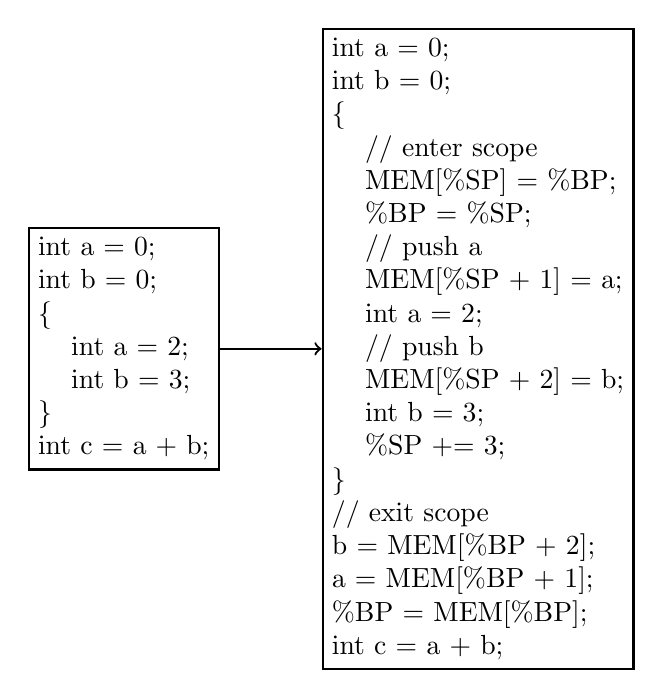
\begin{tikzpicture}[node distance={45mm}, thick, main/.style = {draw}] 
        \node[main, align=left] (Orig) {
            \code{int a = 0;}\\
            \code{int b = 0;}\\
            \code{\{}\\
            \code{\hspace{12pt}int a = 2;}\\
            \code{\hspace{12pt}int b = 3;}\\
            \code{\}}\\
            \code{int c = a + b;}
        };
        \node[main, align=left] (Scoped) [right of=Orig] {
            \code{int a = 0;}\\
            \code{int b = 0;}\\
            \code{\{}\\
            \comment{\hspace{12pt}// enter scope }\\
            \red{\code{\hspace{12pt}MEM[\%SP] = \%BP;}}\\
            \red{\code{\hspace{12pt}\%BP = \%SP;}}\\
            \comment{\hspace{12pt}// push a }\\
            \red{\code{\hspace{12pt}MEM[\%SP + 1] = a;}}\\
            \code{\hspace{12pt}int a = 2;}\\
            \comment{\hspace{12pt}// push b }\\
            \red{\code{\hspace{12pt}MEM[\%SP + 2] = b;}}\\
            \code{\hspace{12pt}int b = 3;}\\
            \red{\code{\hspace{12pt}\%SP += 3;}}\\
            \code{\}}\\
            \comment{// exit scope }\\
            \red{\code{b = MEM[\%BP + 2];}}\\
            \red{\code{a = MEM[\%BP + 1];}}\\
            \red{\code{\%BP = MEM[\%BP];}}\\
            \code{int c = a + b;}
        };
        \draw[->] (Orig) -- (Scoped);
    \end{tikzpicture} 
    \caption{A scope handling example for \CoBBl, where \code{MEM} represents the write-once memory used for stack simulation. Note that this transformation takes place only if \code{a} and \code{b} are selected by \CoBBl's register spilling.}
    \label{fig:continuation-passing}
\end{figure}

\subsection{Lowering segments into constraints} \label{sec:frontend_lowering}
For all non-memory instructions, \CoBBl~reuses the CirC compiler to lower them down to CirC IR. Memory operations in \CoBBl~are divided into two categories: those on the scope stack introduced by register spilling, and those on the virtual memory composed of allocated arrays. Virtual memory operations are expressed as in Buffet \cite{wahby14buffet} in a 4-tuple ($\addr$, $\val$, $\ls$, $\ts$), marking the address, value, whether the operation is a store or load, and the timestamp of the operation. Scope operations are only expressed as ($\addr$, $\val$), as the write-once memory representation ensures that every access to the same address will always yield the same value, regardless of the type of the operation, or when the operation takes place. 